\label{Chapter Conclusion And Future Works}
    \begin{multicols}{2}
        \section{Conclusion And Future Works}
            Future work will be further improved upon by scraping and feeding data from each talent's alternative outfits to our model since each talent has various kinds of outfits and decorations. 
            \autoref{fig:modelvariation} is an example of completely different official outfits for Uruha Rushia.
            \label{Figure Model Variation}
\begin{figure}[H]
    \centering
    \begin{subfigure}{0.17\textwidth}
        \centering
        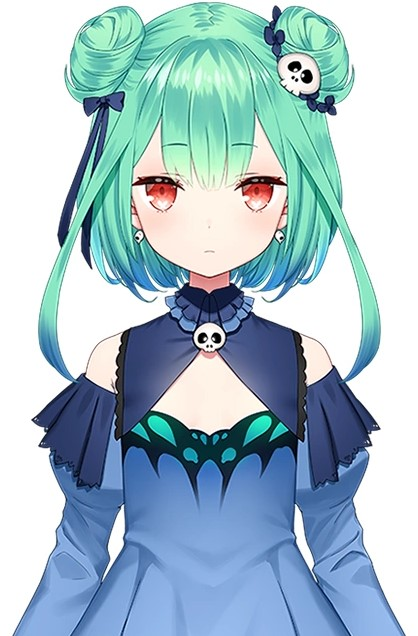
\includegraphics[width=\textwidth]{images/variation/ru1.jpg}
        \caption{Original\cite{rushiaoriginal}}
        \label{fig:ru1}
    \end{subfigure}
    \hfill
    \begin{subfigure}{0.17\textwidth}
        \centering
        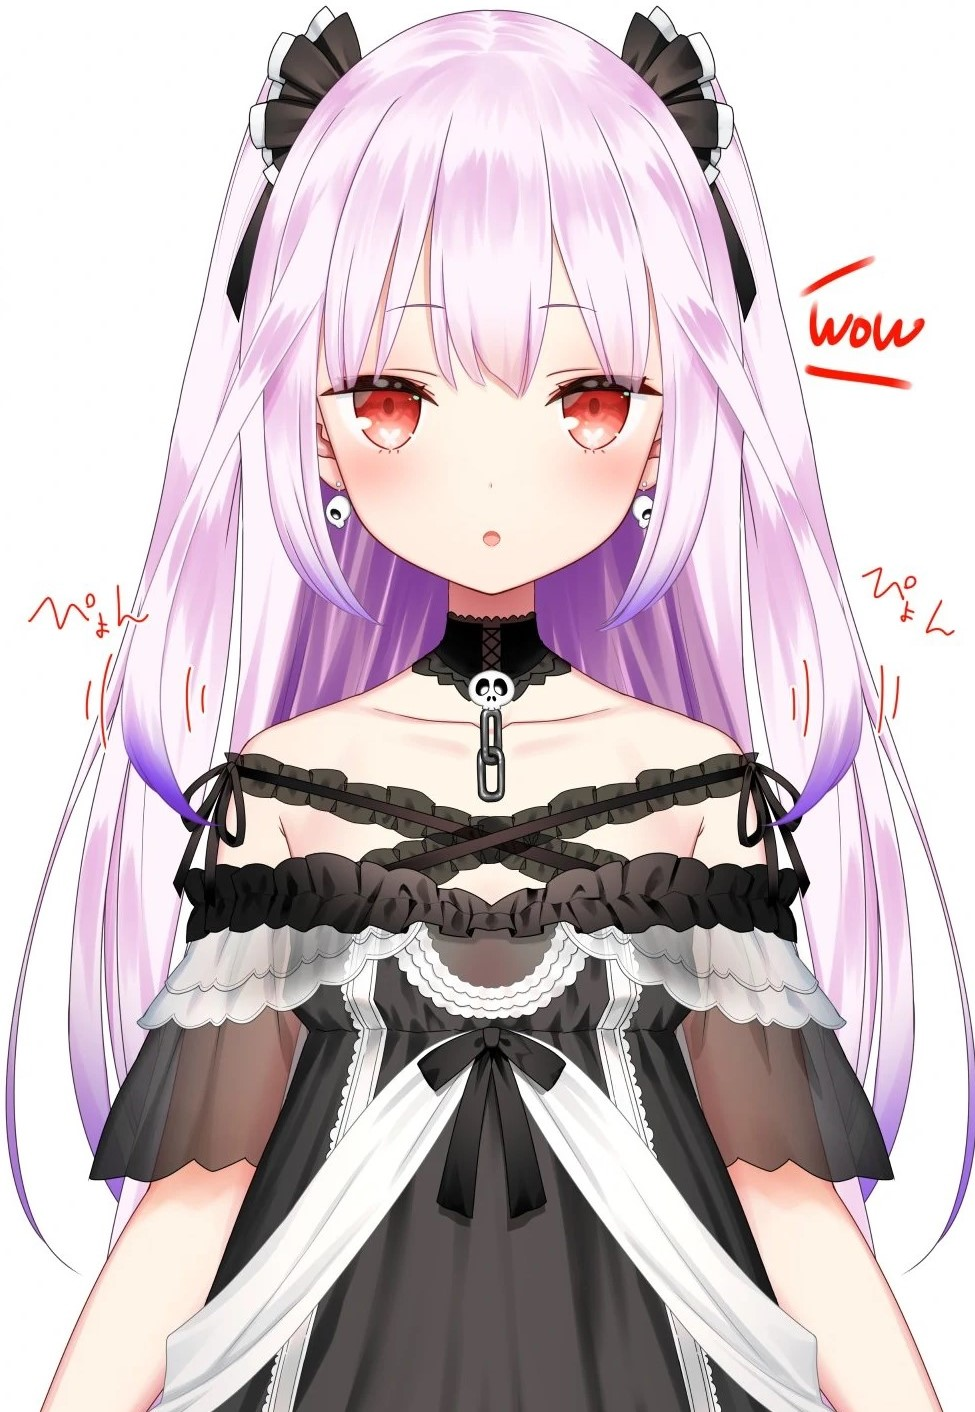
\includegraphics[width=\textwidth]{images/variation/ru2.jpg}
        \caption{Alternative\cite{rushiaalternative}}
        \label{fig:ru2}
    \end{subfigure}
    % \begin{flushleft}
    %     (a) Original outfit\\
    %     (b) Alternative outfit
    % \end{flushleft}
    \caption{Model variation}
    \label{fig:modelvariation}
\end{figure}
            Also, there are many niche cases, such as different angles, real cosplay, characters' outfits swapping, or numerous art styles (\autoref{fig:niche}), that are not in our dataset at the moment.
            
            Furthermore, we hope to develop a tool that will be capable of classifying all virtual YouTubers. Aside from Hololive, there are numerous other agencies (Nijisanji, VShojo, VirtuaReal, etc.) as well as independent VTubers.
        
            Under-sampling is the data splitting method used. However, this approach will not utilize all the available images in the collected dataset. 
            A customized over-sampling algorithm will therefore be included in the upcoming version to resolve this concern. 
            The brief idea is to generate more images using various augmentation techniques to balance the number of labels in each class.

            Last but not least, other helpful augmentation methods (such blur, color channels witching, and etc) will be introduced in the future for further generalization of dataset.
            \begin{figure}[H]
    \centering
    \begin{subfigure}{0.2\textwidth}
        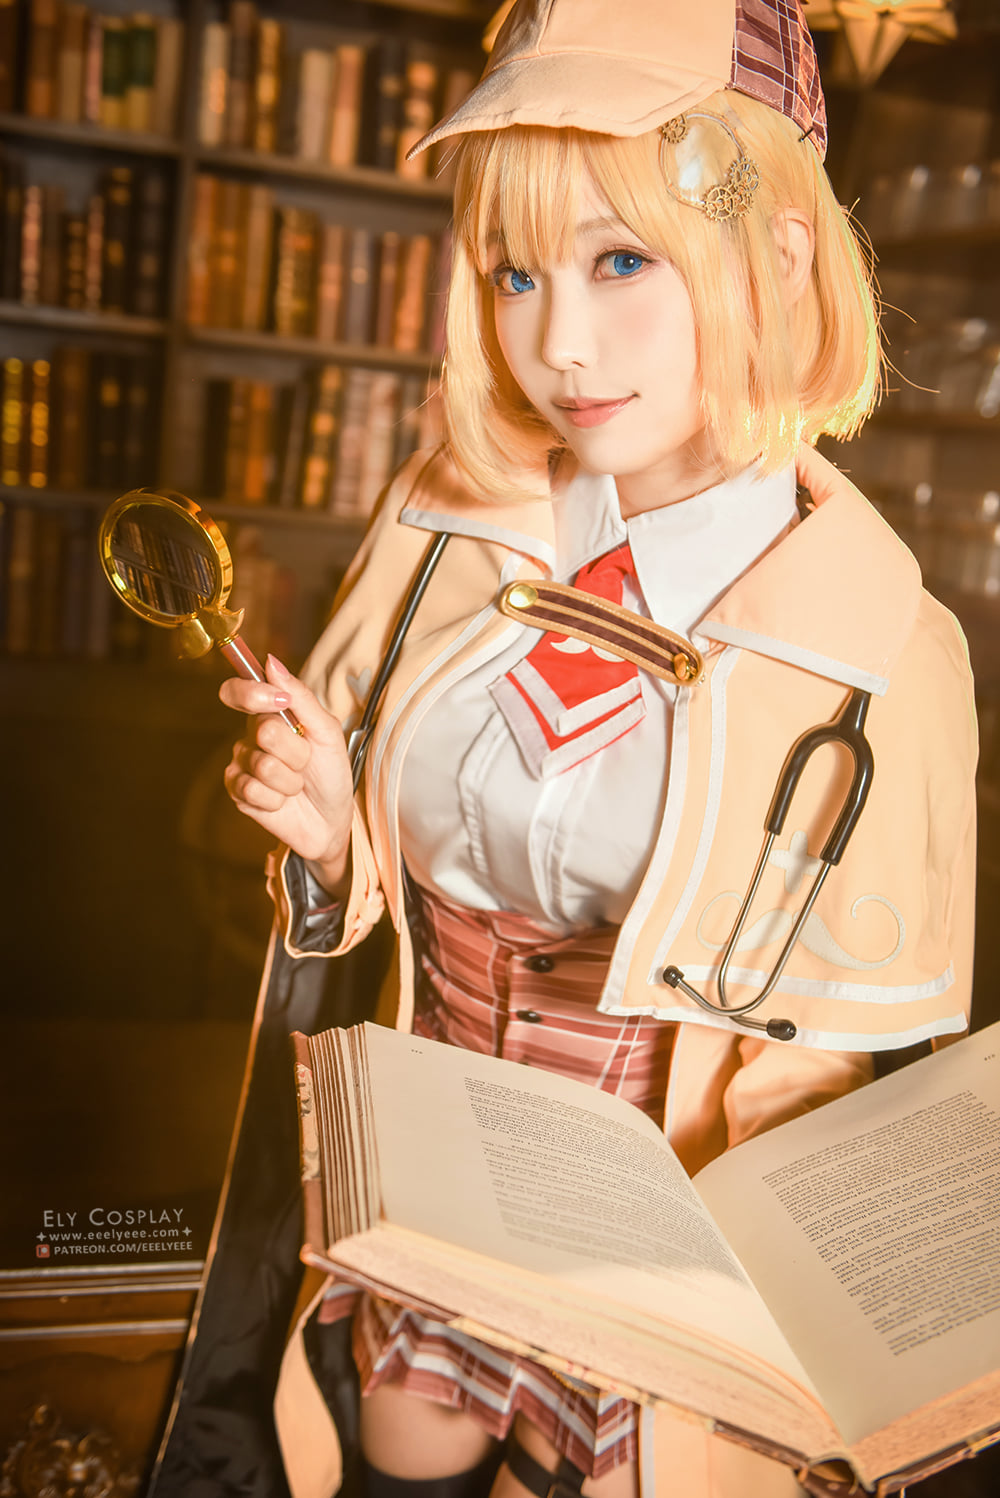
\includegraphics[width=\textwidth]{images/niche/243977316_423878135766209_1700862170532318412_n.jpg}
        \caption{Cosplay\cite{watsoncosply}}
    \end{subfigure}
    \hfill
    \begin{subfigure}{0.2\textwidth}
        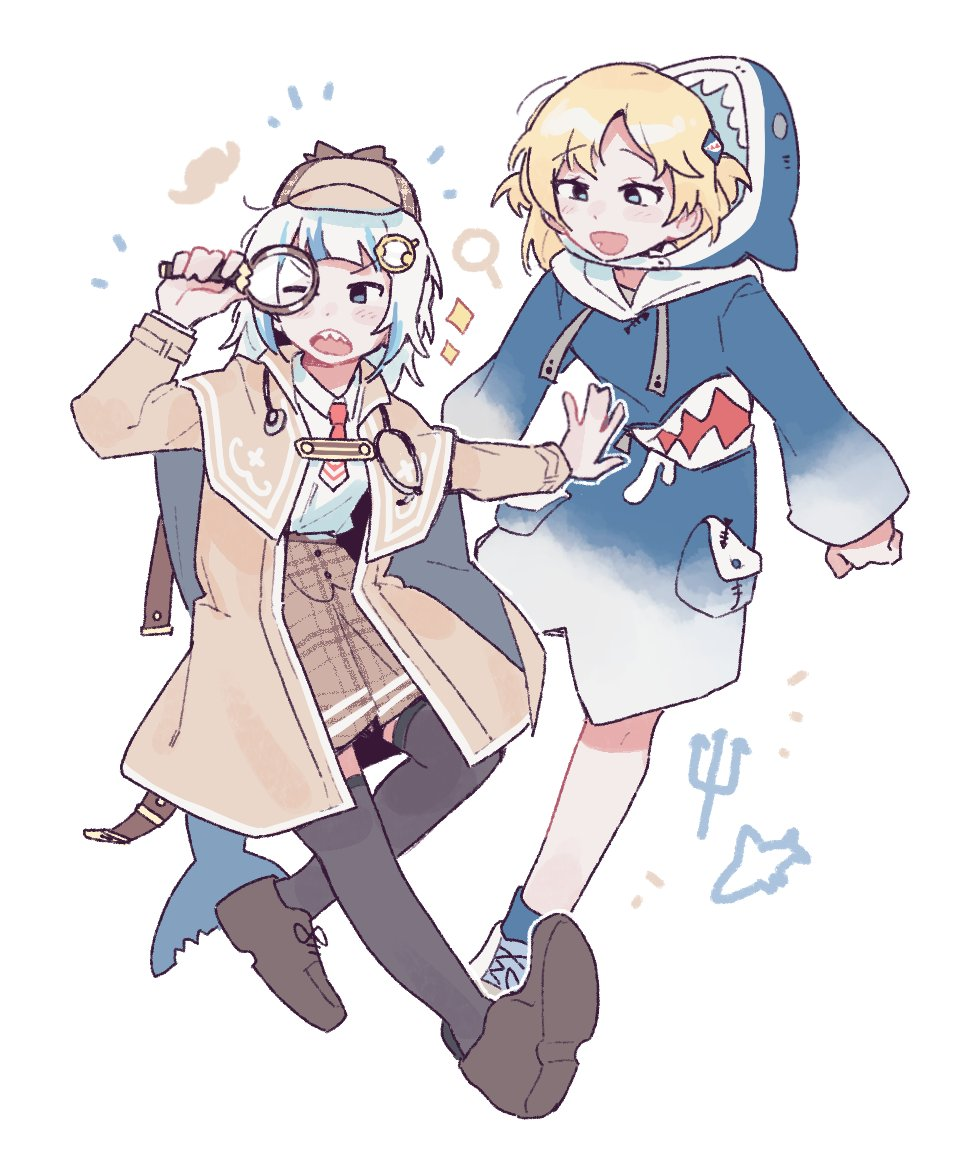
\includegraphics[width=1.3\textwidth]{images/niche/a7u9n4nsnwv51.jpg}
        \caption{Outfit swapping\cite{outfitswapping}}
    \end{subfigure}
    \hfill
    \begin{subfigure}{0.2\textwidth}
        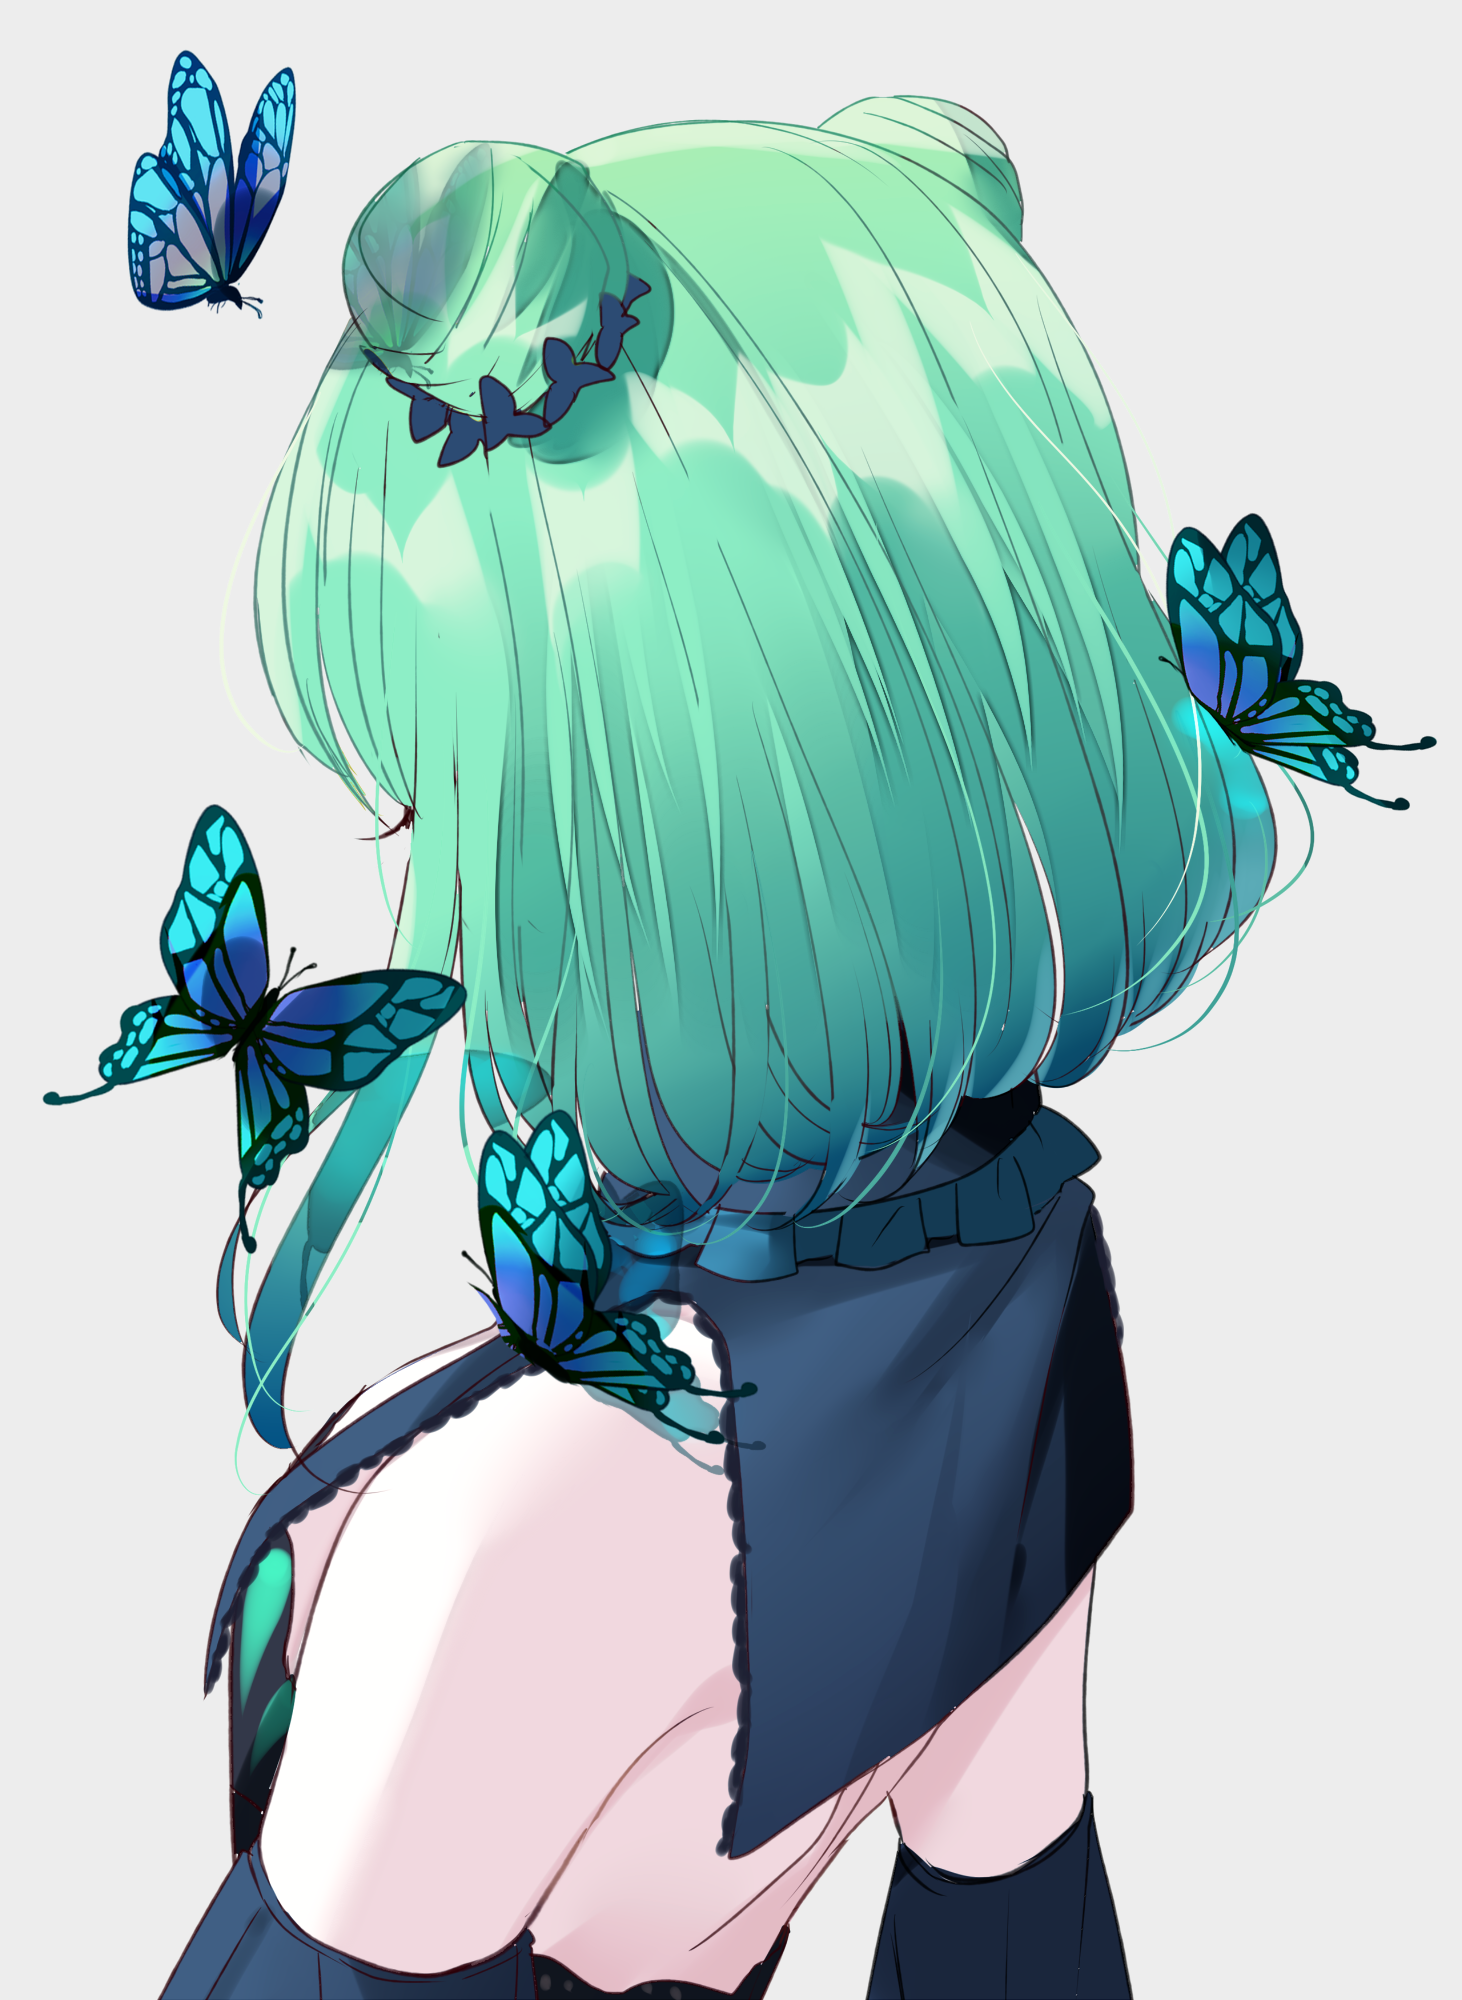
\includegraphics[width=\textwidth]{images/niche/Pixiv-82353068_p5.png}
        \caption{Unusual angle\cite{unusualangle}}
    \end{subfigure}
    \hfill
    \begin{subfigure}{0.2\textwidth}
        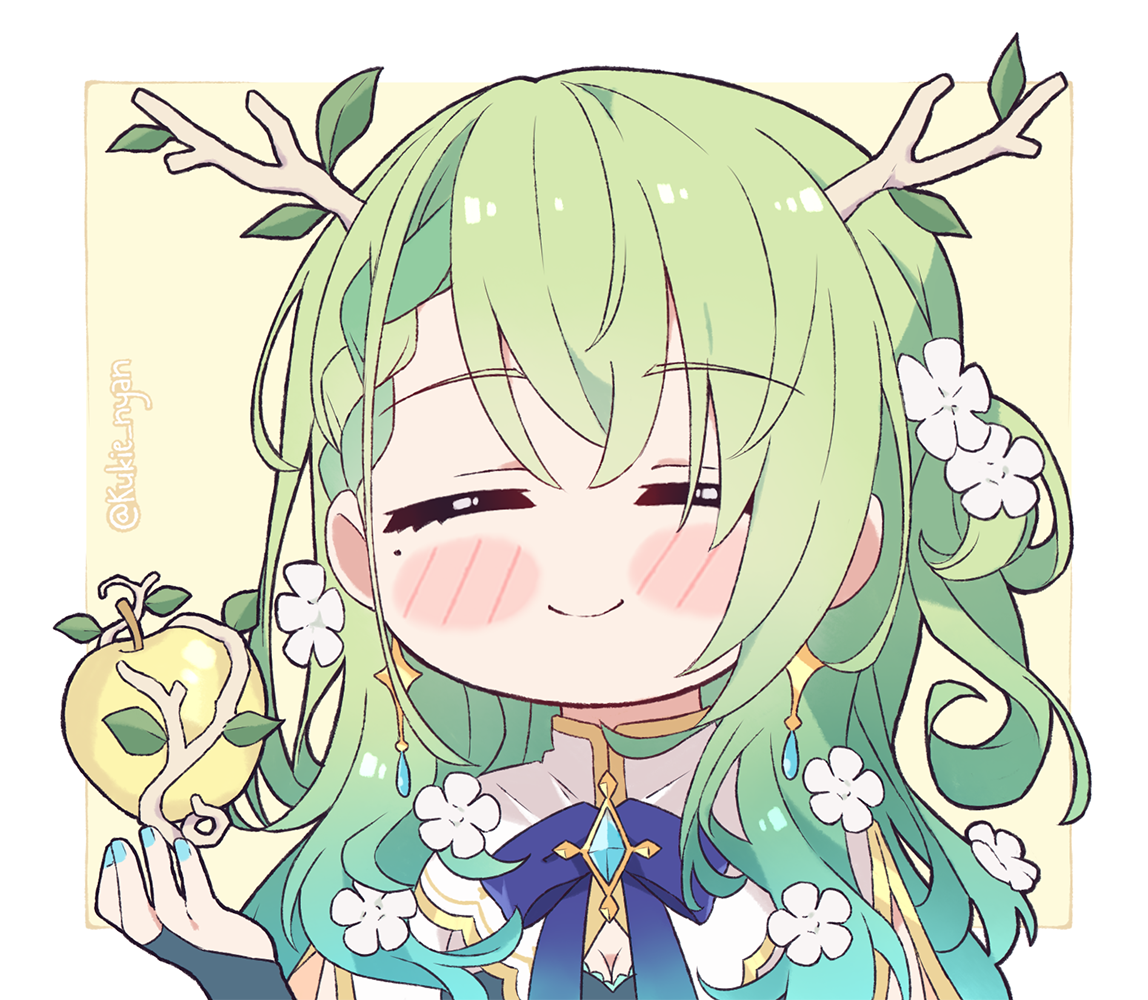
\includegraphics[width=1.5\textwidth]{images/niche/Pixiv-92177593_p0.png}
        \caption{Different artstyle\cite{chibi}}
    \end{subfigure}
    \hfill
    \caption{Uncovered situations}
    \label{fig:niche}
\end{figure}

    \end{multicols}
% \clearpage